\documentclass[]{report}

\usepackage{amsmath}
\usepackage{bm}
\usepackage{graphicx}

\graphicspath{ {images/} }

\title{CSCI 567 HW \# 3}
\author{Mohmmad Suhail Ansari \\ USC ID: 8518586692\\e-mail: mohmmada@usc.edu}

\begin{document}

\maketitle

\paragraph{Sol. 1.1}
	Given, 
	\[ E[\beta] = \frac{1}{n} \sum_{i = 1}^{N} {(y_i - x_i^T \beta)}^2 + \lambda {\|\beta\|}_2^2\]

	We can write from definition of X
	\[ \sum^N (y_i - x_i^T \beta)^2 = {\| (\textbf{y} - X \beta)\|}^2 = (\textbf{y} - X \beta)^T (\textbf{y} - X \beta)\]

	substituting in the first equation

	\[ E[\beta] = \frac{1}{n} (\textbf{y} - X \beta)^T (\textbf{y} - X \beta) + \lambda \beta^T \beta \]

	taking partial derivative w.r.t. $\beta$, we get

	\[ \frac{\partial{E[\beta]}}{\partial{\beta}} = \frac{2}{n} [-X^T \textbf{y} + X^T X \beta] + 2 \lambda \beta = 0\]
	\[ = -X^T \textbf{y} + X^T X \beta + n \lambda \beta \]
	\[ X^T \textbf{y} = (X^T X + n \lambda I_D) \beta \]
	\[ \hat{\beta}_\lambda = (X^T X + n \lambda I_D)^{-1} X^T \textbf{y} \]


	Since, $\epsilon$ is normally distributed, we have 
	\[ y = \mathcal{N}(X^T \beta^*, \delta^2 I)\]
	and since $\hat{y} = X^T \hat{\beta}_\lambda$, we have 
	\[ \hat{\beta}_\lambda = \mathcal{N}((X^T X + n \lambda I_D)^{-1} X^T X^T \beta^*, (X^T X + n \lambda I_D)^{-1} X^T \delta^2 (X^T X + n \lambda I_D)^{-1} )\]
	

\paragraph{Sol. 1.2}
	
	From 1.2, let $L = X^T X$, then if we replace it in the $\hat{\beta}_\lambda$, we get 
	\[ \hat{\beta}_\lambda = (L + n \lambda I) X^T y \]
	\[ = (L(I + n\lambda L^{-1}))^{-1} L [L^{-1} X^T y] \]
	\[ = (I + n \lambda L^{-1})^{-1} L^{-1} L [(X^T X)^{-1} X^T y]\]
	and since, $(X^T X)^{-1} X^T y = \beta^*$, we get 
	\[ \hat{\beta}_\lambda = (I + n\lambda L^{-1})^{-1} \beta^* \]

	Now,
	\[ E[ x^T \hat{\beta}_\lambda ] - x^T \beta^* = X^T (I + n\lambda L^{-1})^{-1} \beta^* - X^T \beta^* \]
	\[ = X^T (I + n\lambda (X^T X)^{-1})^{-1} - I) \beta^* \]

\paragraph{Sol. 1.3}
	
	N/A

\paragraph{Sol. 1.4}
	
	N/A


\paragraph{Sol. 2.1}
	using Mercer's theorem we can write for any function $f(\cdot)$
	\[ \int_{x, x'} k_3 (x, x') f(x) f(x') dx dx' \]
	\[ = \int_{x, x'} (a_1 k_1 (x, x') + a_2 k_2 (x, x') ) f(x) f(x') dx dx' \]
	\[ = \int_{x, x'} a_1 k_1 (x, x') f(x) f(x') dx dx' + \int_{x, x'} a_2 k_2 (x, x') f(x) f(x') dx dx' \]
	and since, we know that $k_1 (\cdot, \cdot)$ and $k_2 (\cdot, \cdot)$ are valid kernel functions, then 
	\[ \int_{x, x'} k_3 (x, x') f(x) f(x') dx dx' \geq 0 \]
	and hence, $k_3 (\cdot, \cdot)$ is a valid kernel function.

\paragraph{Sol. 2.2}
	
	For a feature map $\phi$ we know that a valid kernel is defined as
	\[ k(x, x') = \langle \phi(x), \phi(x') \rangle \]
	so we if we use the feature map $\phi: x \rightarrow f(x)$, then 
	\[ k_4(x, x')  = {\langle \phi(x), \phi(x') \rangle}_{\chi^\phi} \]
	\[ = f(x) f(x') \]
	because $f(x)$ is real valued and hence, $k_4(x, x') = f(x) f(x')$ is a valid kernel.

	%if $f(\cdot)$ is a real valued function then using Mercer's theorem we can write
	%\[ \int_{x, x'}  k_4 (x, x') f(x) f(x') dx dx' \]
	%\[ = \int_{x, x'} f(x) f(x') f(x) f(x') dx dx' \]
	%\[ = \int_{x, x'} (f(x))^2 (f(x'))^2 dx dx' \]
	%and since $(f(\cdot))^2 \geq 0$, therefore
	%\[ \int_{x, x'}  k_4 (x, x') f(x) f(x') dx dx' \geq 0 \]
	%and hence, $k_4$ is a valid kernel function.

\paragraph{Sol. 2.3}
	Let, $\phi_1$ and $\phi_2$ be feature map of $k_1$ and $k_2$ respectively and let $f_i (x)$ and $g_i (x)$ be $i^{th}$ feature value for 
	$\phi_1$ and $\phi_2$ respectively, then by definition of $k_5$, we can write
	\[ k_5 (x, x') = k_1 (x, x') k_2 (x, x') \]
	\[ = {\phi_1 (x)}^T \phi_1 (x') {\phi_2 (x)}^T \phi(x') \]
	\[ = (\sum_{i} f_i (x) f_i (x')) (\sum_{j} g_j (x) g_j (x')) \]
	\[ = \sum_i \sum_j (f_i (x) g_j (x)) (f_j (x') g_j (x'))\]
	so now, we can define a feature map $\phi_3$ where its $i^{th}$ feature is defined as $h_{i, j}(x) = f_i (x) g_j (x)$. Which gives us
	\[ k_5 (x, x') = {\phi_3 (x)}^T \phi_3 (x')\]
	Also, $k_5$ is symmetric since both $k_1$ and $k_2$ are symmetric, i.e.
	\[ k_5 (x, x') = k_1 (x, x') k_2 (x, x') \]
	\[ = k_1 (x', x) k_2 (x', x) \]
	\[ = k_5 (x', x) \]
	therefore $k_5$ is a valid kernel function.

\paragraph{Sol. 3.1}
	From the text, we can write the objective function as 
	\[ \epsilon(w) = \sum_n (y_i - w^T x_i)^2 + \lambda {\| w \|}_2^2 \]
	we know that
	\begin{align}
    	w^T x_i &= \begin{bmatrix}
           w_1 \\
           w_2 \\
           \vdots \\
           w_D
         \end{bmatrix} \begin{bmatrix}x_{i1} x_{i2} \cdots x_{iD} \end{bmatrix}
  	\end{align}
  	\[ = \sum_j^D w_j x_{ij} = \sum_j^D x_{ij} w_j \]
  	\[ = x_i^T w \]

  	Now, if $\textbf{y} = [y_1 \, y_2 \, y_3 \cdots \, y_N]$ and
  	\begin{align}
    	X &= \begin{bmatrix}
           x_{11} & x_{21} \cdots x_{N1}\\
           x_{12} & x_{22} \cdots x_{N2}\\
           x_{13} & x_{23} \cdots x_{N3}\\
           \vdots & \vdots  \\
           x_{1D} & x_{2D} \cdots x_{ND}
         \end{bmatrix}
  	\end{align}
  	
  	we write
  	\[ \sum_n (y_i - w^T x_i)^2 = \| \textbf{y} - Xw \|_2^2 \]
  	
  	then we have 
  	\[ \epsilon(w) = \|\textbf{y} - Xw\|_2^2 + \lambda \| w\|_2^2 \]

	taking partial derivative w.r.t $w$, we get 
	\[ \frac{\partial{\epsilon(w)}}{\partial{w}} = 2 X^T (\textbf{y} - Xw) + 2\lambda w = 0\]
	%%now, we can write $w^T x_i = x_i^T w$,
	%%\[ = -\sum_n (y_i x_i) + (\sum_n x_i^T x_i) w + \lambda w = 0 \]
	%%we can write $\sum_n (y_i x_i) = yX = X^T y$ and $\sum_n x_i^T x_i = X^T X$
	%%\[ = -X^T \textbf{y} + X^T X w + \lambda w = 0 \]
	%%\[ = -X^T \textbf{y} + (X^T X + \lambda I_D ) w = 0\]
	\begin{equation}
		 w^* = {(X^T X + \lambda I_D)}^{-1} X^T \textbf{y}
	\end{equation}

\paragraph{Sol. 3.2}	
	we know
	\[ w^* =  {(X^T X + \lambda I_D)}^{-1} X^T \textbf{y} \]
	 
	also, 
	\[ (X^T X + \lambda I_D) X^T = X^T X X^T + \lambda X^T = X^T (X X^T + \lambda I_N)\] 
	multiplying both sides with $(X^T X + \lambda I_D)^{-1}$ on left and $(X X^T + \lambda I_N)^{-1} \textbf{y}$ on right, we get
	\[ X^T (X X^T + \lambda I_N)^{-1} \textbf{y} = (X^T X + \lambda I_D)^{-1} X^T \textbf{y} \]

	using the above equation in $w^{*}$, we get
	\[ w^{*} = X^T (X X^T + \lambda I_N)^{-1} \textbf{y}\]

	Now, if we substitute $X$ with $\mathbf{\Phi} (x)$ (because dimensions of $XX^T$ and $\mathbf{\Phi}(x) {\mathbf{\Phi}(x)}^T$ is $N \times N$)
	therefore we can write 
	\[ w^* = \mathbf{\Phi}^T {(\mathbf{\Phi} \mathbf{\Phi}^T + \lambda I_N)}^{-1} \textbf{y} \]
	
\paragraph{Sol. 3.3}
	\[ \hat{y} = w^{*T}\phi(x)\]
	\[ = {[\mathbf{\Phi}^T {(\mathbf{\Phi} \mathbf{\Phi}^T + \lambda I_N)}^{-1} \textbf{y}]}^{T} \phi(x)\]
	\[ = y^T {((\mathbf{\Phi} \mathbf{\Phi}^T + \lambda I_N)^T)}^{-1} \mathbf{\Phi} \phi(x) \]
	\[ = y^T {(\mathbf{\Phi}^T \mathbf{\Phi} + \lambda I_N)}^{-1} \mathbf{\Phi} \phi(x) \]
	
	we also have, 
	\begin{align}
    	\mathbf{\Phi} \phi(x) &= \begin{bmatrix}
           \phi(x_1)^T \phi(x) \\
           \phi(x_2)^T \phi(x) \\
           \phi(x_3)^T \phi(x) \\
           \vdots  \\
           \phi(x_N)^T \phi(x)
         \end{bmatrix} = \kappa(x)
  	\end{align}
	substituting value of $K$ and $\kappa(x)$ in $\hat{y}$, we get 
	\[ \hat{y} = \textbf{y}^T (K + \lambda I_N)^{-1} \kappa(x) \]

\paragraph{Sol. 3.4}
	The time complexity for both is $O(N^3)$, but in Ridge Regression there are two instances of matrix multiplication and one inversion, taking
	$O(N^3)$ whereas Kernel Ridge Regression only calculate matrix inverse once.


\paragraph{Sol. 4.1}
	As we can see from the graph below the positive examples are \textbf{not} linearly separable from negative examples.

\paragraph{Sol. 4.2}
	As observed from values of the transformed feature space a hyper plane in the dimension of $(x_1 x_2)$ feature separates the points, therefore we have
	\[ w = [0 \quad 0 \quad 0 \quad 1]\]

\paragraph{Sol. 4.3}
	Adding (0.5, 0.5) as a negative example will prevent the positive and negative examples to no longer be linearly separable.	

\paragraph{Sol. 4.4}
	This feature transformation corresponds to the the $K(x, x')$ given as 
	\[ K(x, x') = 1 + x^2 + {x'}^2 + (x x' )^2\]


\paragraph{Sol. 5} $\newline$
	
	\textbf{(1)} Since, $C \rightarrow \infty$, the penalty for misclassification is really high, i.e. the decision will perfectly divide the points. However, since the points are linearly inseparable the decision boundary is indeterminable (or at least it is not linear). 
	\\

	\textbf{(2)}
	For $C \approx 0$, means the misclassification penalty is small and the decision boundary would mis-classify some points. But a linear can be found (shown in figure below)
	\\

	\textbf{(3)}
	The case with $C \approx 0$ will perform better than case with $C \rightarrow \infty$, since a large value of C will choose a smaller-margin hyperplane compared to small value of C, so small-margin hyperplane might not generalize the vectors enough, i.e. the accuracy for $C \rightarrow \infty$ will be high for training data, but it might perform well for test (unseen) data, whereas the $C \approx 0$ will generalize the vectors enough to perform well for test data.
	\\

	\textbf{(4)}
	Since, the data is already linearly inseparable and and for large $C$ there needs to be a decision boundary which should separate points with minimal misclassification so any point in or near the cluster or ``$-$'' points will still lead to same decision boundary (shown below).
	\\

	\textbf{(5)}
	A point far from the ``$-$'' cluster will change the decision boundary significantly since the decision boundary should not misclassify (large C) this point ans must include the new point on the correct side of the decision boundary.
	\\

	\begin{center}
		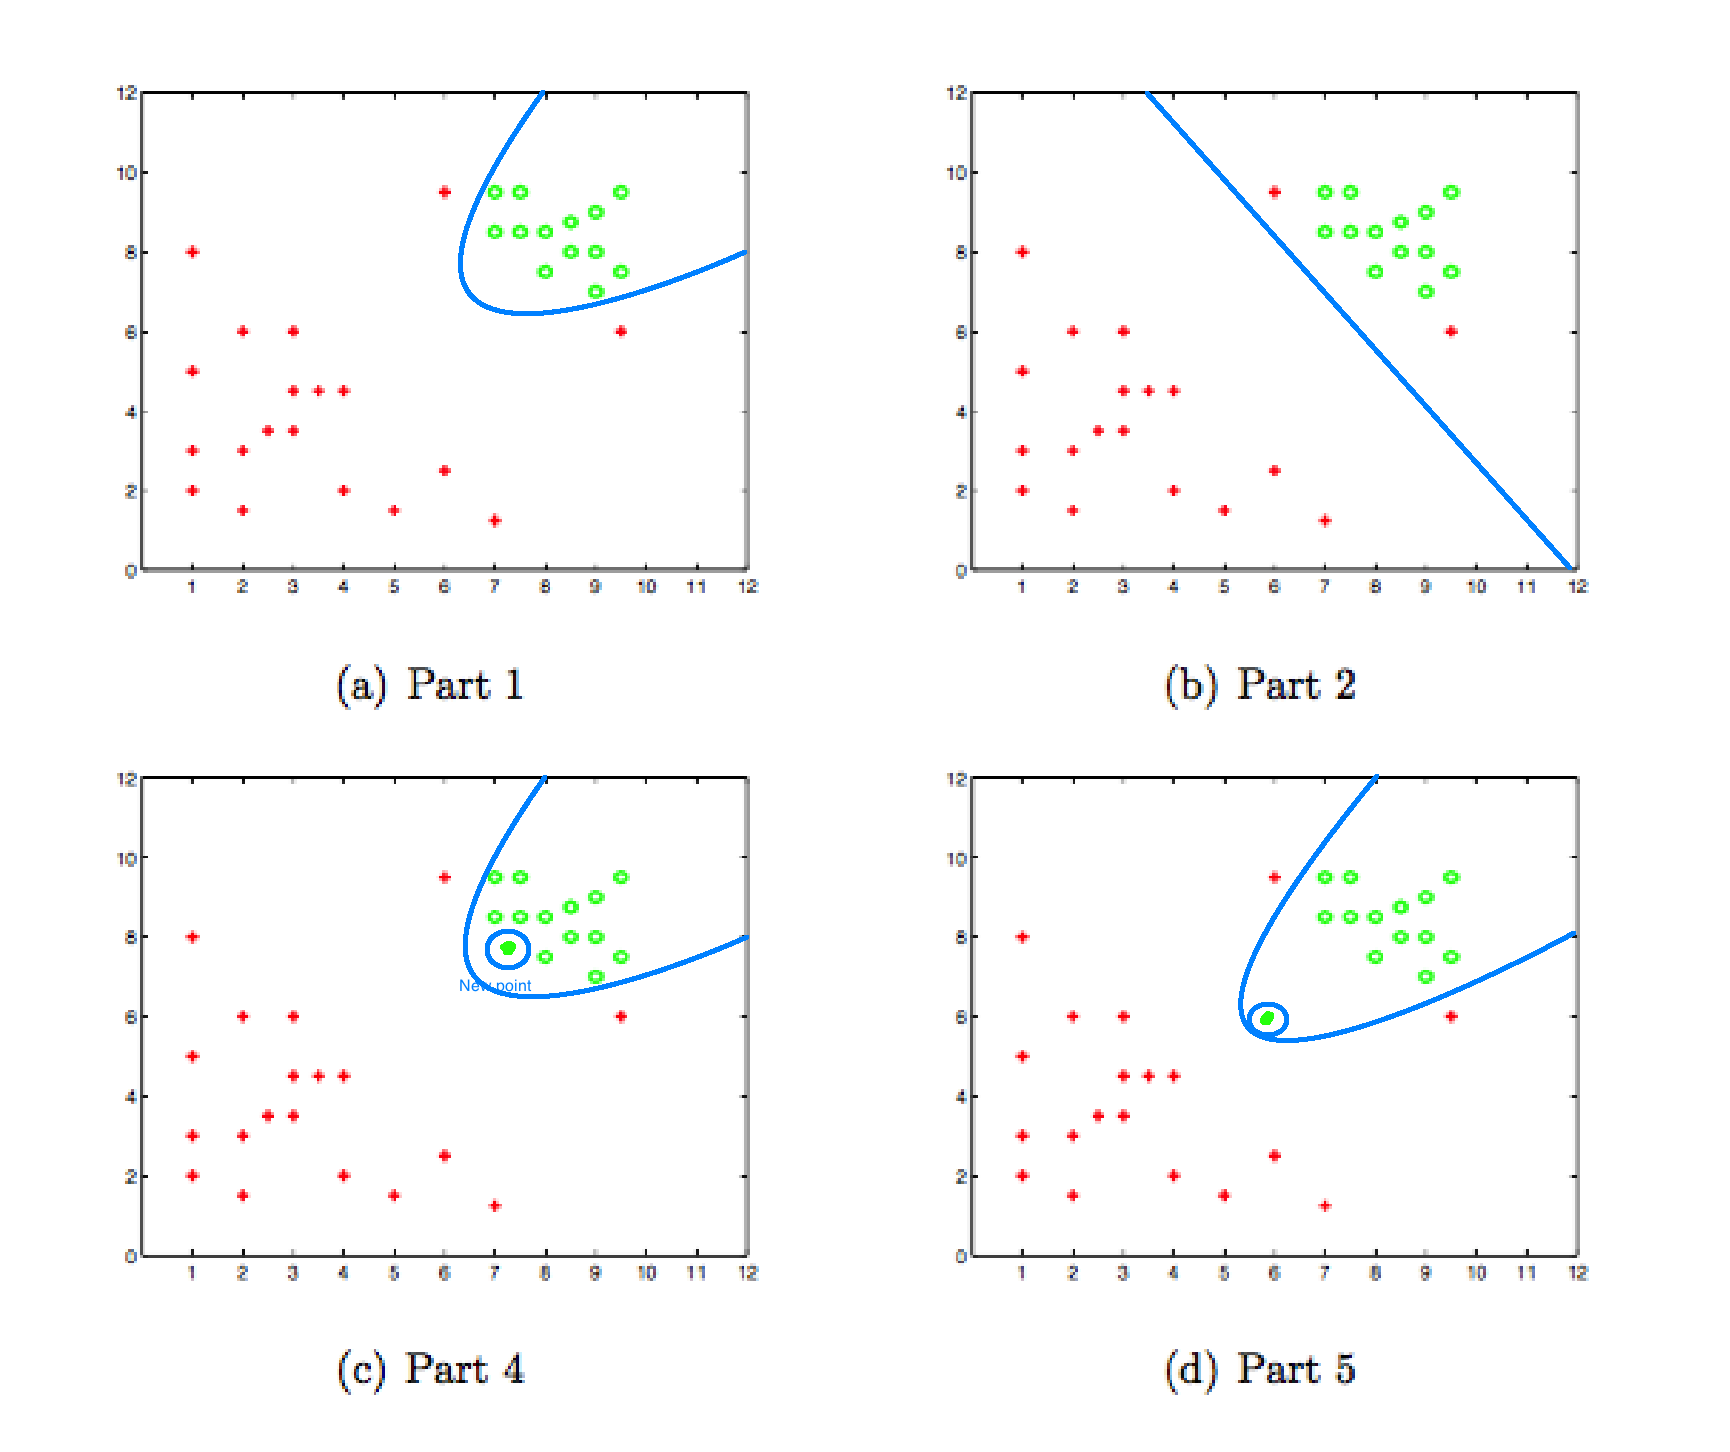
\includegraphics[width=\textwidth]{Problem-5}
	\end{center}

\paragraph{Sol. 6}
\subparagraph{1.a}
	For sample size of n = 10, we have the following plot
	\begin{center}
		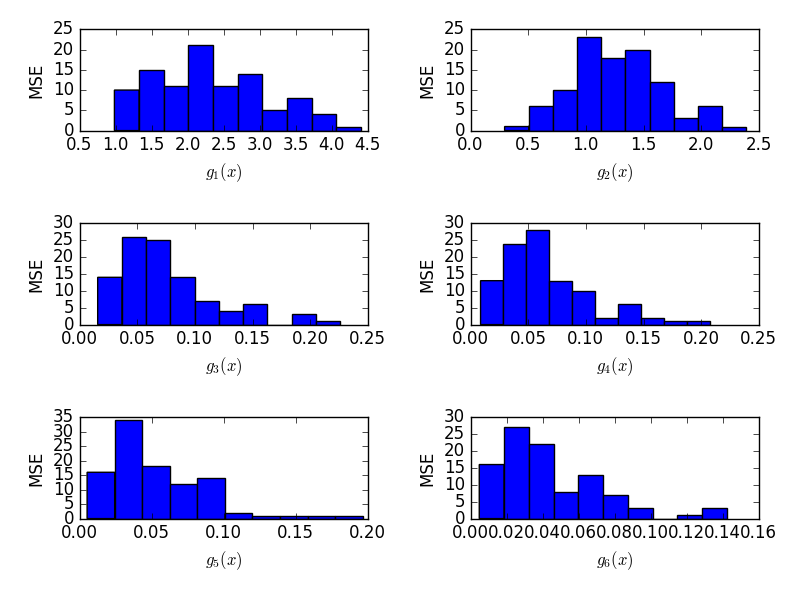
\includegraphics[width=\textwidth]{fig_10_MSE}
	\end{center}
	and the bias and variance are

	\begin{center}
		\begin{tabular}{c|c|c}
		\hline
		 $g(x)$     &   $Var[\hat{y}]$ &   ${Bias}^2$ \\
		\hline
		 $g_0 (x)$ &      0           & 0.00835376 \\
		 $g_1 (x)$ &      0 		  & 0.0010114999 \\
		 $g_2 (x)$ &      0.0129696   & 0.0010114995 \\
		 $g_3 (x)$ &      0.0129735   & 0.0010114991 \\
		 $g_4 (x)$ &      0.0129809   & 0.0010114983 \\
		 $g_5 (x)$ &      0.0129812   & 0.0010114976 \\
		\hline
		\end{tabular}
	\end{center}

\subparagraph{1.b}
	For sample size of n = 100, we have the following plot
	\begin{center}
		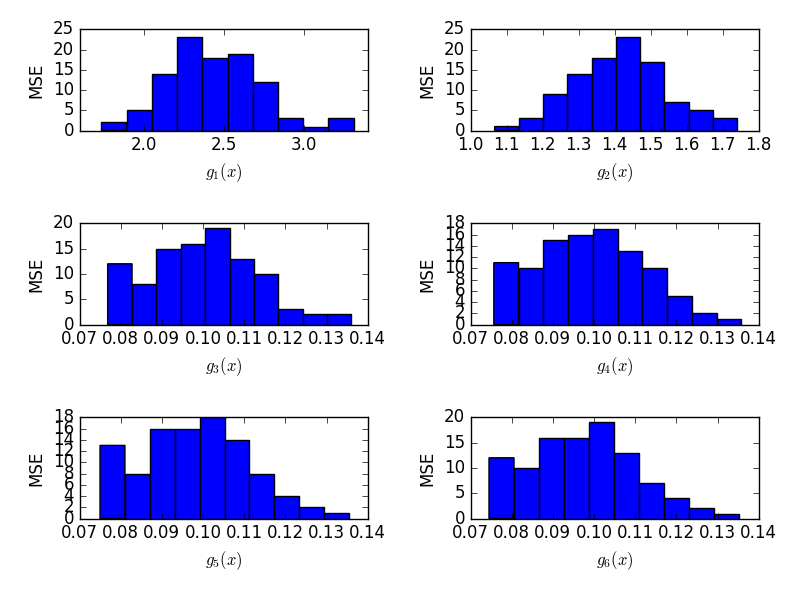
\includegraphics[width=\textwidth]{fig_100_MSE}
	\end{center}

	and the bias and variance are

	\begin{center}
		\begin{tabular}{c|c|c}
			\hline
			 $g(x)$     &   $Var[\hat{y}]$ &   ${Bias}^2$ \\
			\hline
			 $g_0 (x)$ &      0           & 0.0100663   \\
			 $g_1 (x)$ &      0  		  & 0.00020746359 \\
			 $g_2 (x)$ &      0.0114071   & 0.00020746354 \\
			 $g_3 (x)$ &      0.011429    & 0.00020746349 \\
			 $g_4 (x)$ &      0.0114578   & 0.00020746346 \\
			 $g_5 (x)$ &      0.011458    & 0.00020746345 \\
			\hline
			\end{tabular}
	\end{center}

\subparagraph{1.c}
	If we plot the ${Bias}^2$ against $Var[\hat{y}]$ we see that with increasing complexity, the ${Bias}^2$ decreases and $Var[\hat{y}]$
	increases.

	For Sample Size (n) = 10
	\begin{center}
		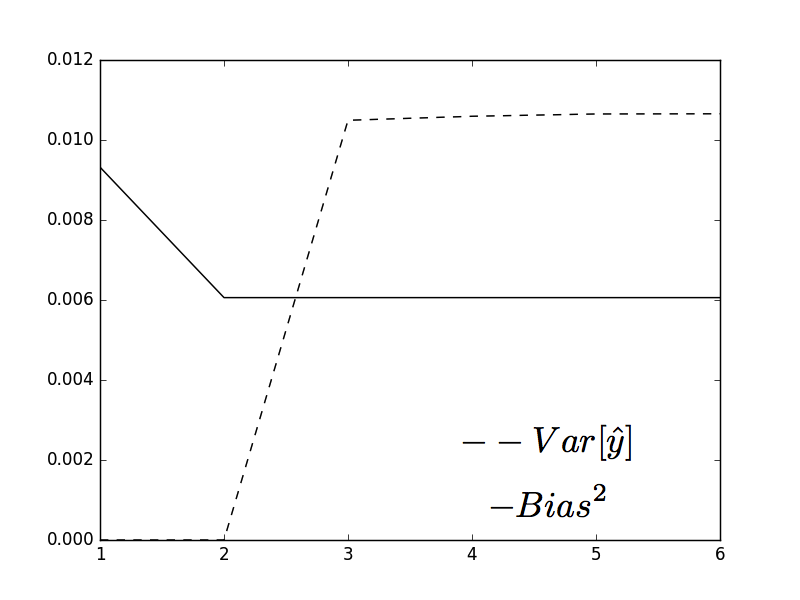
\includegraphics[width=\textwidth]{fig_10_BV}
	\end{center}

	For Sample Size (n) = 100
	\begin{center}
		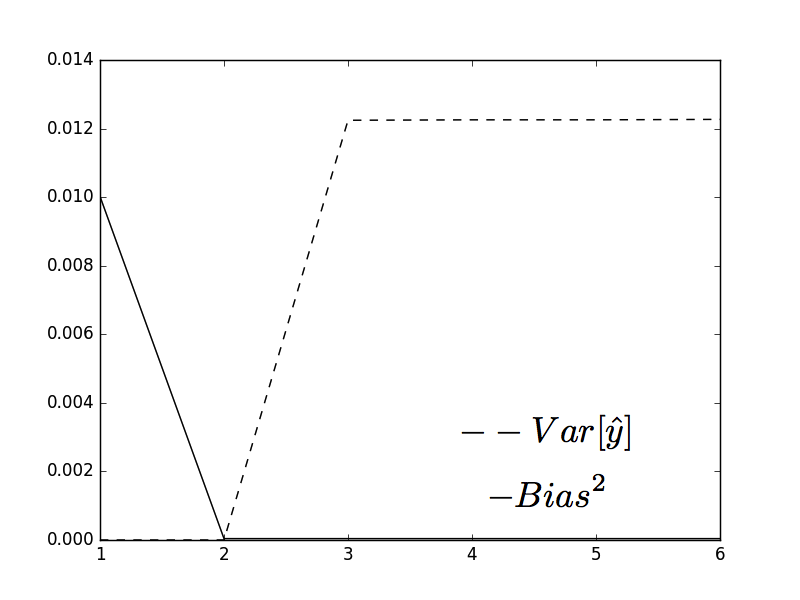
\includegraphics[width=\textwidth]{fig_100_BV}
	\end{center}

	We can also observe that with increase in sample size, both ${Bias}^2$ and $Var[\hat{y}]$ decreases.

\subparagraph{1.d}
	For each value of $\lambda$ we get the values for $Bias^2$ and $Var[\hat{y}]$ as 
	\begin{center}
		\begin{tabular}{c|c|c}
			\hline
			           $\lambda$ &    $Var[\hat{y}]$ &          $Bias^2$ \\
			\hline
			 0.001 & 1.339555842497451 & 1.335753691359456 \\
			 0.003 & 1.339555198601041 & 1.335753691360410 \\
			 0.010 & 1.339547874313111 & 1.335753691371258 \\
			 0.030 & 1.339483487636583 & 1.335753691466629 \\
			 0.1   & 1.338751426233234 & 1.335753692551133 \\
			 0.3   & 1.332342280730491 & 1.335753702058702 \\
			 1.0   & 1.262651053579910 & 1.335753806797648 \\
			\hline
		\end{tabular}
	\end{center}

	We can see from the plots below that $Var[\hat{y}$ decreases with increasing $\lambda$, whereas $Bias^2$ increases with increasing $\lambda$.

	\begin{center}
		
		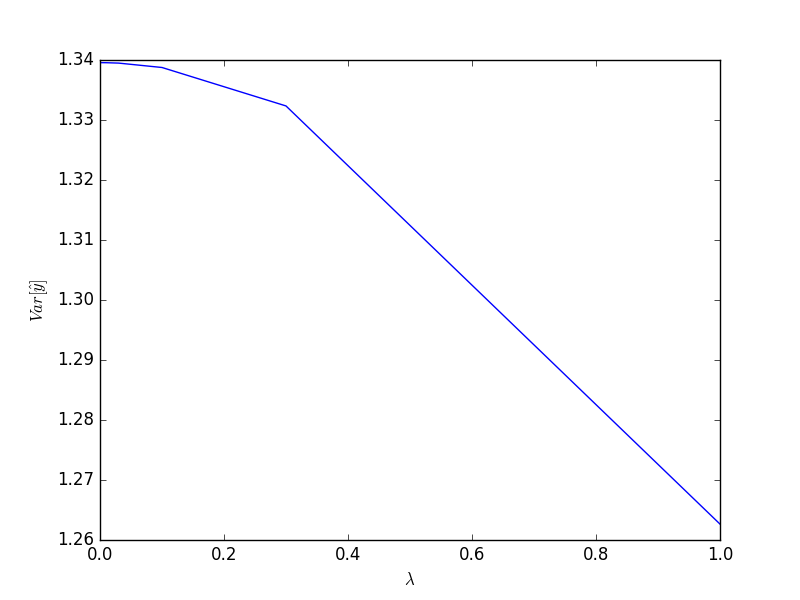
\includegraphics[width=\textwidth]{var_lambda}
		\[ Var[\hat{y}] \]
	\end{center}
	
	\begin{center}
		
		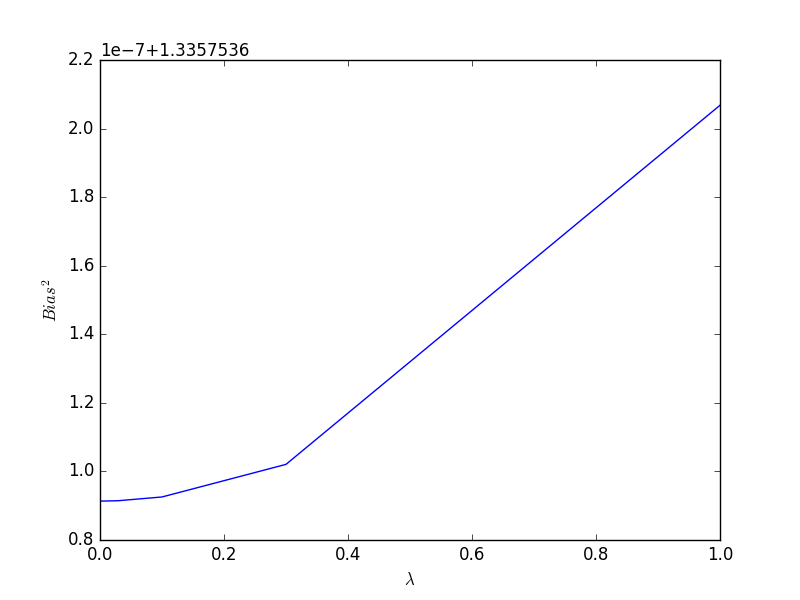
\includegraphics[width=\textwidth]{bias_lambda}
		\[ Bias^2 \]
	\end{center}

\subparagraph{Use linear SVM in LIBSVM}
	\begin{center}
		\begin{tabular}{l|c|c}
			\hline
			    C     & 3-Fold Cross Validation Accuracy  & Execution Time \\
			    \hline
			    $4^{-6}$     & 55.75\%     & 0m0.687s      \\
			    $4^{-5}$     & 55.75\%     & 0m0.654s      \\
			    $4^{-4}$     & 55.75\%     & 0m0.666s      \\
			    $4^{-3}$     & 71.55\%     & 0m0.711s      \\
			    $4^{-2}$     & 91.55\%     & 0m0.533s      \\
			    $4^{-1}$     & 91.8\%      & 0m0.338s      \\
			    $4^{2}$      & 96.35\%     & 0m0.204s      \\
			    $4^{0}$      & 94.05\%     & 0m0.239s      \\
			    $4^{1}$      & 95.5\%      & 0m0.206s      \\
			\hline
		\end{tabular}
	\end{center}
	Average Training Time : 0.4708s

\newpage



\subparagraph{Use Kernel SVM in LIBSVM}

	\begin{center}			
		Polynomial Kernel
			\begin{tabular}{lr|c|c|c}
			\hline
			 C      &   degree & 3-Fold Cross Validation Accuracy   & Execution Time   \\
			\hline
			 $4^{-3}$ &        1 & 55.75\%                             & 0m0.727s         \\
			 $4^{-3}$ &        2 & 55.75\%                             & 0m0.697s         \\
			 $4^{-3}$ &        3 & 55.75\%                             & 0m0.717s         \\
			 $4^{-2}$ &        1 & 90.25\%                             & 0m0.581s         \\
			 $4^{-2}$ &        2 & 89\%                                & 0m0.688s         \\
			 $4^{-2}$ &        3 & 76.7\%                              & 0m0.801s         \\
			 $4^{-1}$ &        1 & 91.2\%                              & 0m0.360s         \\
			 $4^{-1}$ &        2 & 92.05\%                             & 0m0.441s         \\
			 $4^{-1}$ &        3 & 92.05\%                             & 0m0.513s         \\
			 $4^{0}$  &        1 & 92.75\%                             & 0m0.248s         \\
			 $4^{0}$  &        2 & 93.2\%                              & 0m0.292s         \\
			 $4^{0}$  &        3 & 92.7\%                              & 0m0.366s         \\
			 $4^{1}$  &        1 & 94.45\%                             & 0m0.200s         \\
			 $4^{1}$  &        2 & 94.95\%                             & 0m0.217s         \\
			 $4^{1}$  &        3 & 95.2\%                              & 0m0.233s         \\
			 $4^{2}$  &        1 & 94.5\%                              & 0m0.236s         \\
			 $4^{2}$  &        2 & 95.9\%                              & 0m0.191s         \\
			 $4^{2}$  &        3 & 96.15\%                             & 0m0.193s         \\
			 $4^{3}$  &        1 & 94.25\%                             & 0m0.209s         \\
			 $4^{3}$  &        2 & 96.65\%                             & 0m0.182s         \\
			 $4^{3}$  &        3 & 97\%                                & 0m0.195s         \\
			 $4^{4}$  &        1 & 94.45\%                             & 0m0.337s         \\
			 $4^{4}$  &        2 & 97\%                                & 0m0.188s         \\
			 $4^{4}$  &        3 & 97.05\%                             & 0m0.175s         \\
			 $4^{5}$  &        1 & 94.15\%                             & 0m0.544s         \\
			 $4^{5}$  &        2 & 96.75\%                             & 0m0.186s         \\
			 $4^{5}$  &        3 & 96.55\%                             & 0m0.203s         \\
			 $4^{6}$  &        1 & 94.2\%                              & 0m2.278s         \\
			 $4^{6}$  &        2 & 96.95\%                             & 0m0.240s         \\
			 $4^{6}$  &        3 & 96.7\%                              & 0m0.184s         \\
			 $4^{7}$  &        1 & 94.2\%                              & 0m5.259s         \\
			 $4^{7}$  &        2 & 96.7\%                              & 0m0.265s         \\
			 $4^{7}$  &        3 & 96.7\%                              & 0m0.188s         \\
			 \hline
			\end{tabular}
		\end{center}

		Average Training Time : 0.5555s

		\newpage
	\begin{center}		
		RBF Kernel
			\begin{tabular}{l|l|c|c}
			\hline
			 C      & $\gamma$   & 3-Fold Cross Validation Accuracy   & Execution Time   \\
			\hline
			 $4^{-3}$ & $4^{-7}$   & 55.75\%                             & 0m0.717s         \\
			 $4^{-3}$ & $4^{-6}$   & 55.75\%                             & 0m0.760s         \\
			 $4^{-3}$ & $4^{-5}$   & 55.75\%                             & 0m0.773s         \\
			 $4^{-3}$ & $4^{-4}$   & 55.75\%                             & 0m0.724s         \\
			 $4^{-3}$ & $4^{-3}$   & 56\%                                & 0m0.800s         \\
			 $4^{-3}$ & $4^{-2}$   & 87.55\%                             & 0m0.658s         \\
			 $4^{-3}$ & $4^{-1}$   & 60.6\%                              & 0m0.704s         \\
			 $4^{-2}$ & $4^{-7}$   & 55.75\%                             & 0m0.676s         \\
			 $4^{-2}$ & $4^{-6}$   & 55.75\%                             & 0m0.749s         \\
			 $4^{-2}$ & $4^{-5}$   & 55.75\%                             & 0m0.883s         \\
			 $4^{-2}$ & $4^{-4}$   & 64.4\%                              & 0m0.738s         \\
			 $4^{-2}$ & $4^{-3}$   & 90.55\%                             & 0m0.862s         \\
			 $4^{-2}$ & $4^{-2}$   & 92.2\%                              & 0m0.415s         \\
			 $4^{-2}$ & $4^{-1}$   & 92.95\%                             & 0m0.595s         \\
			 $4^{-1}$ & $4^{-7}$   & 55.75\%                             & 0m0.673s         \\
			 $4^{-1}$ & $4^{-6}$   & 55.75\%                             & 0m0.739s         \\
			 $4^{-1}$ & $4^{-5}$   & 66.55\%                             & 0m0.741s         \\
			 $4^{-1}$ & $4^{-4}$   & 90.85\%                             & 0m0.890s         \\
			 $4^{-1}$ & $4^{-3}$   & 91.35\%                             & 0m0.370s         \\
			 $4^{-1}$ & $4^{-2}$   & 93.2\%                              & 0m0.292s         \\
			 $4^{-1}$ & $4^{-1}$   & 95.7\%                              & 0m0.391s         \\
			 $4^{0}$  & $4^{-7}$   & 55.75\%                             & 0m0.760s         \\
			 $4^{0}$  & $4^{-6}$   & 67.8\%                              & 0m0.697s         \\
			 $4^{0}$  & $4^{-5}$   & 91.05\%                             & 0m0.524s         \\
			 $4^{0}$  & $4^{-4}$   & 91.35\%                             & 0m0.588s         \\
			 $4^{0}$  & $4^{-3}$   & 93.55\%                             & 0m0.229s         \\
			 $4^{0}$  & $4^{-2}$   & 96.05\%                             & 0m0.207s         \\
			 $4^{0}$  & $4^{-1}$   & 97.15\%                             & 0m0.281s         \\
			 $4^{1}$  & $4^{-7}$   & 68.05\%                             & 0m0.836s         \\
			 $4^{1}$  & $4^{-6}$   & 90.9\%                              & 0m0.670s         \\
			 $4^{1}$  & $4^{-5}$   & 91.4\%                              & 0m0.391s         \\
			 $4^{1}$  & $4^{-4}$   & 93.3\%                              & 0m0.300s         \\
			 $4^{1}$  & $4^{-3}$   & 94.85\%                             & 0m0.185s         \\
			 $4^{1}$  & $4^{-2}$   & 96.8\%                              & 0m0.165s         \\
			 $4^{1}$  & $4^{-1}$   & 96.95\%                             & 0m0.263s         \\
			 $4^{2}$  & $4^{-7}$   & 90.9\%                              & 0m1.207s         \\
			 $4^{2}$  & $4^{-6}$   & 91.5\%                              & 0m0.537s         \\
			 $4^{2}$  & $4^{-5}$   & 93.35\%                             & 0m0.237s         \\
			 $4^{2}$  & $4^{-4}$   & 94.6\%                              & 0m0.205s         \\
			 $4^{2}$  & $4^{-3}$   & 96\%                                & 0m0.182s         \\
			 $4^{2}$  & $4^{-2}$   & 97.15\%                             & 0m0.163s         \\
			 $4^{2}$  & $4^{-1}$   & 96.7\%                              & 0m0.263s         \\
			 \hline
			\end{tabular}

			Continued... \newline

			\begin{tabular}{l|l|c|c}
			\hline
			 C      & $\gamma$   & 3-Fold Cross Validation Accuracy   & Execution Time   \\
			\hline
			 $4^{3}$  & $4^{-7}$   & 91.5\%                              & 0m0.429s         \\
			 $4^{3}$  & $4^{-6}$   & 93.45\%                             & 0m0.335s         \\
			 $4^{3}$  & $4^{-5}$   & 94.45\%                             & 0m0.278s         \\
			 $4^{3}$  & $4^{-4}$   & 94.65\%                             & 0m0.194s         \\
			 $4^{3}$  & $4^{-3}$   & 96.7\%                              & 0m0.168s         \\
			 $4^{3}$  & $4^{-2}$   & 97\%                                & 0m0.167s         \\
			 $4^{3}$  & $4^{-1}$   & 96.7\%                              & 0m0.249s         \\
			 $4^{4}$  & $4^{-7}$   & 93.45\%                             & 0m0.277s         \\
			 $4^{4}$  & $4^{-6}$   & 94.45\%                             & 0m0.266s         \\
			 $4^{4}$  & $4^{-5}$   & 94.5\%                              & 0m0.260s         \\
			 $4^{4}$  & $4^{-4}$   & 95.65\%                             & 0m0.196s         \\
			 $4^{4}$  & $4^{-3}$   & 97.3\%                              & 0m0.174s         \\
			 $4^{4}$  & $4^{-2}$   & 96.85\%                             & 0m0.180s         \\
			 $4^{4}$  & $4^{-1}$   & 96.7\%                              & 0m0.242s         \\
			 $4^{5}$  & $4^{-7}$   & 94.45\%                             & 0m0.236s         \\
			 $4^{5}$  & $4^{-6}$   & 94.5\%                              & 0m0.262s         \\
			 $4^{5}$  & $4^{-5}$   & 94.55\%                             & 0m0.297s         \\
			 $4^{5}$  & $4^{-4}$   & 96.7\%                              & 0m0.232s         \\
			 $4^{5}$  & $4^{-3}$   & 96.9\%                              & 0m0.203s         \\
			 $4^{5}$  & $4^{-2}$   & 96.85\%                             & 0m0.169s         \\
			 $4^{5}$  & $4^{-1}$   & 96.7\%                              & 0m0.249s         \\
			 $4^{6}$  & $4^{-7}$   & 94.45\%                             & 0m0.199s         \\
			 $4^{6}$  & $4^{-6}$   & 94.75\%                             & 0m0.191s         \\
			 $4^{6}$  & $4^{-5}$   & 95.65\%                             & 0m0.434s         \\
			 $4^{6}$  & $4^{-4}$   & 97.3\%                              & 0m0.311s         \\
			 $4^{6}$  & $4^{-3}$   & 97\%                                & 0m0.225s         \\
			 $4^{6}$  & $4^{-2}$   & 96.85\%                             & 0m0.166s         \\
			 $4^{6}$  & $4^{-1}$   & 96.7\%                              & 0m0.260s         \\
			 $4^{7}$  & $4^{-7}$   & 94.6\%                              & 0m0.264s         \\
			 $4^{7}$  & $4^{-6}$   & 94.45\%                             & 0m0.277s         \\
			 $4^{7}$  & $4^{-5}$   & 96.5\%                              & 0m0.484s         \\
			 $4^{7}$  & $4^{-4}$   & 96.85\%                             & 0m0.422s         \\
			 $4^{7}$  & $4^{-3}$   & 97\%                                & 0m0.225s         \\
			 $4^{7}$  & $4^{-2}$   & 96.85\%                             & 0m0.156s         \\
			 $4^{7}$  & $4^{-1}$   & 96.7\%                              & 0m0.238s         \\
			 \hline
			\end{tabular}

	\end{center}

	Average Training Time : 0.415s \newline

	We find that the best 3-Fold Cross Validation accuracy we can achieve it using an RBF Kernel with parameters $C = 4^6$ and $\gamma = 4^{-4}$.
	After running the libsvm with appropriate parameters we get the classification accuracy = 49.85\%.


\end{document}